\documentclass[aspectratio=1610]{beamer}
\usepackage[utf8]{inputenc}
\usepackage[T1]{fontenc}
\usepackage{amsmath, amssymb}
\usepackage{array}
\usepackage{tabularx}
\usepackage{booktabs}
\usepackage{tikz}

\title{zk-STARK}
\subtitle{Skalabilni i transparentni dokazi nultog znanja}
\author{Nikola Milošević 1063/2024}
\date{\today}

% Koristi kolegin wildcat templejt ako postoji u projektu.
% Ako se fajl kompajlira van projekta, koristi se rezervna Beamer tema.
\IfFileExists{beamerthemewildcat.sty}{
	\usetheme[color=nudarkblue,numbering=progressbar]{wildcat}
}{
	\usetheme{Madrid}
	\setbeamertemplate{navigation symbols}{}
	\setbeamertemplate{footline}[frame number]
	\newenvironment{pblock}[1]{\begin{block}{##1}}{\end{block}}
}

\begin{document}
	
	\begin{frame}
		\titlepage
	\end{frame}
	
	\begin{frame}{Sadržaj}
		\tableofcontents
	\end{frame}
	
	% ------------------------------------------------------------
	\section{Motivacija}
	% ------------------------------------------------------------
	
	\begin{frame}{Gde se uklapa zk-STARK?}
		\begin{itemize}
			\item U prethodnom delu obrađeni su dokazi nultog znanja i zk-SNARK sistemi.
			\item zk-SNARK omogućava kratak dokaz i brzu verifikaciju, ali mnoge konstrukcije koriste \textit{trusted setup}.
			\item zk-STARK pokušava da zadrži ideju dokaza nultog znanja, ali uz:
			\begin{itemize}
				\item transparentno podešavanje,
				\item skalabilnu verifikaciju,
				\item sigurnost zasnovanu pre svega na heš funkcijama.
			\end{itemize}
		\end{itemize}
	\end{frame}
	
	\begin{frame}{Šta znači zk-STARK?}
		\begin{pblock}{Definicija}
			\textbf{zk-STARK} je skraćenica od \textit{Zero-Knowledge Scalable Transparent Argument of Knowledge}.
		\end{pblock}
		
		\begin{itemize}
			\item \textbf{Zero-Knowledge} — dokaz ne otkriva tajni svedok.
			\item \textbf{Scalable} — verifikator proverava mnogo manje od celog izračunavanja.
			\item \textbf{Transparent} — nema faze poverljivog podešavanja.
			\item \textbf{Argument of Knowledge} — validan dokaz implicira posedovanje odgovarajućeg svedoka.
		\end{itemize}
		
	\end{frame}
	
	\begin{frame}{Motivacioni problem}
		\begin{itemize}
			\item Neka organizacija poseduje poverljive podatke $D$.
			\item Nad njima izvršava program $C$ i objavljuje rezultat:
		\end{itemize}
		
		\[
		y = C(D)
		\]
		
		\begin{pblock}{Pitanje}
			Kako verifikator može da proveri da je rezultat zaista ispravan, a da ne vidi poverljive podatke i ne ponavlja celo izračunavanje?
		\end{pblock}
		
		\begin{itemize}
			\item Naivna provera: verifikator dobija $D$ i ponovo računa $C(D)$.
			\item Problem: narušava privatnost i može biti preskupo.
			\item zk-STARK: šalje se dokaz $\pi$, ne kompletan skup podataka.
		\end{itemize}
	\end{frame}
	
	\begin{frame}{Primer: poverljiva DNK baza}
		\begin{pblock}{Ideja iz originalnog STARK rada}
			Policija želi da dokaže da se DNK profil određene osobe ne nalazi u poverljivoj bazi, bez objavljivanja baze i bez oslanjanja na spoljnog revizora.
		\end{pblock}
		
		\begin{itemize}
			\item Baza DNK profila je poverljiva.
			\item Javnost želi dokaz da je pretraga korektno izvršena.
			\item Verifikator ne treba da vidi bazu niti da sam pretražuje sve zapise.
			\item zk-STARK omogućava dokaz integriteta izračunavanja nad tajnim podacima.
		\end{itemize}
	\end{frame}
	
	% ------------------------------------------------------------
	\section{Osnovne osobine}
	% ------------------------------------------------------------
	
	\begin{frame}{Transparentnost}
		\begin{itemize}
			\item Kod mnogih zk-SNARK konstrukcija postoji faza poverljivog podešavanja.
			\item U toj fazi nastaju javni parametri, ali i tajne pomoćne vrednosti.
			\item Te tajne vrednosti se neformalno nazivaju \textit{toxic waste}.
			\item Ako bi ih neko sačuvao, potencijalno bi mogao da pravi lažne dokaze.
		\end{itemize}
		
		\begin{pblock}{zk-STARK pristup}
			Parametri su javni; sistem koristi javnu nasumičnost i kriptografske heš funkcije. Ne postoji tajni parametar koji mora biti uništen.
		\end{pblock}
	\end{frame}
	
	\begin{frame}{Postkvantna orijentacija}
		\begin{itemize}
			\item Mnogi zk-SNARK sistemi koriste eliptičke krive i bilinearna uparivanja.
			\item Njihova sigurnost je povezana sa problemom diskretnog logaritma.
		\end{itemize}
		
		\[
		Q = kP
		\]
		
		\begin{itemize}
			\item Šorov algoritam bi na dovoljno snažnom kvantnom računaru ugrozio diskretni logaritam.
			\item zk-STARK se ne oslanja na tu pretpostavku.
			\item Umesto toga koristi heš funkcije i Reed--Solomonove kodove.
		\end{itemize}
		
		\begin{pblock}{Zaključak}
			Zato se zk-STARK opisuje kao \textit{plausibly post-quantum secure}, ali to nije apsolutna garancija protiv svih budućih napada.
		\end{pblock}
	\end{frame}
	
	\begin{frame}{Skalabilnost}
		\begin{itemize}
			\item Dokazivač mora da obradi izvršavanje programa.
			\item Verifikator ne treba da ponovi celo izvršavanje.
			\item Ideja je da verifikator proveri samo mali broj nasumično izabranih mesta.
		\end{itemize}
		
		\begin{center}
			\begin{tabular}{c|c}
				\textbf{Uloga} & \textbf{Tipičan cilj} \\
				\hline
				Dokazivač & približno $O(n\log n)$ \\
				Verifikator & polilogaritamski u $n$ \\
				Komunikacija & manja od celog traga izvršavanja
			\end{tabular}
		\end{center}
		
		\begin{pblock}{Važno}
			Ovo su pojednostavljene procene. Konkretne performanse zavise od širine traga, stepena ograničenja, heš funkcije i parametara protokola.
		\end{pblock}
	\end{frame}
	
	% ------------------------------------------------------------
	\section{Kako STARK funkcioniše}
	% ------------------------------------------------------------
	
	\begin{frame}{Tok STARK protokola}
		\begin{center}
			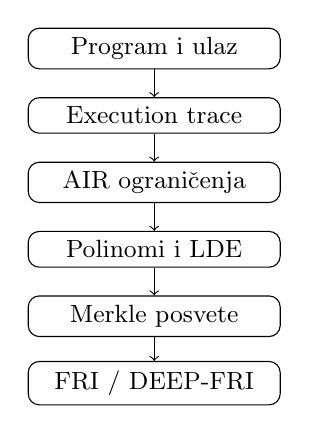
\begin{tikzpicture}[node distance=0.85cm, every node/.style={font=\small}]
				\node[draw, rounded corners, align=center, minimum width=3.2cm] (program) {Program i ulaz};
				\node[draw, rounded corners, below of=program, align=center, minimum width=3.2cm] (trace) {Execution trace};
				\node[draw, rounded corners, below of=trace, align=center, minimum width=3.2cm] (air) {AIR ograničenja};
				\node[draw, rounded corners, below of=air, align=center, minimum width=3.2cm] (poly) {Polinomi i LDE};
				\node[draw, rounded corners, below of=poly, align=center, minimum width=3.2cm] (commit) {Merkle posvete};
				\node[draw, rounded corners, below of=commit, align=center, minimum width=3.2cm] (fri) {FRI / DEEP-FRI};
				\draw[->] (program) -- (trace);
				\draw[->] (trace) -- (air);
				\draw[->] (air) -- (poly);
				\draw[->] (poly) -- (commit);
				\draw[->] (commit) -- (fri);
			\end{tikzpicture}
		\end{center}
	\end{frame}
	
	\begin{frame}{Execution trace}
		\begin{pblock}{Ideja}
			Izvršavanje programa se predstavlja kao tabela međustanja.
		\end{pblock}
		
		\begin{itemize}
			\item Svaki red predstavlja jedan korak izvršavanja.
			\item Kolone predstavljaju registre, memorijske vrednosti ili druge promenljive stanja.
			\item Ako je trag ispravan, onda svaki prelaz između redova zadovoljava pravila programa.
		\end{itemize}
		
		\begin{center}
			\begin{tabular}{c|c}
				Korak $i$ & Vrednost $x_i$ \\
				\hline
				0 & $x_0$ \\
				1 & $x_1$ \\
				2 & $x_2$ \\
				$\vdots$ & $\vdots$ \\
				$n$ & $x_n$
			\end{tabular}
		\end{center}
	\end{frame}
	
	\begin{frame}{AIR: algebrarski opis izvršavanja}
		\begin{pblock}{AIR}
			\textit{Algebraic Intermediate Representation} opisuje ispravno izvršavanje programa pomoću polinomskih ograničenja.
		\end{pblock}
		
		\begin{itemize}
			\item \textbf{Granična ograničenja}: početne i završne vrednosti.
			\item \textbf{Tranziciona ograničenja}: pravila prelaska između susednih stanja.
		\end{itemize}
		
		\begin{pblock}{Primer}
			Ako program računa
			\[
			x_{i+1} = x_i^2 + c,
			\]
			onda je tranziciono ograničenje
			\[
			x_{i+1} - x_i^2 - c = 0.
			\]
		\end{pblock}
	\end{frame}
	
	\begin{frame}{Od traga do polinoma}
		\begin{itemize}
			\item Svaka kolona traga posmatra se kao skup evaluacija polinoma.
			\item Za domen izvršavanja
		\end{itemize}
		
		\[
		H = \{\omega^0, \omega^1, \ldots, \omega^{n-1}\}
		\]
		
		\begin{itemize}
			\item postoji polinom $f(X)$ takav da:
		\end{itemize}
		
		\[
		f(\omega^i) = x_i.
		\]
		
		\begin{itemize}
			\item Dokazivač zatim računa evaluacije na većem domenu.
			\item To se zove \textbf{low-degree extension} (LDE).
			\item LDE se oslanja na Reed--Solomonove kodove.
		\end{itemize}
	\end{frame}
	
	\begin{frame}{Zašto proširenje domena?}
		\begin{itemize}
			\item Vektor evaluacija polinoma niskog stepena ponaša se kao Reed--Solomonova kodna reč.
			\item Ako dokazivač menja vrednosti, rezultat postaje daleko od validne kodne reči.
			\item Verifikator zatim može probabilistički da proveri bliskost sa polinomom niskog stepena.
		\end{itemize}
		
		\begin{pblock}{FFT}
			Interpolacija i evaluacija polinoma nad struktuiranim domenima efikasno se izvršavaju brzim furijeovim transformacijama nad konačnim poljima.
		\end{pblock}
		
	\end{frame}
	
	\begin{frame}{Merkle posvete}
		\begin{itemize}
			\item Dokazivač ima veliki niz evaluacija.
			\item Ne šalje ih sve verifikatoru.
			\item Umesto toga gradi Merklovo stablo.
		\end{itemize}
		
\begin{center}
	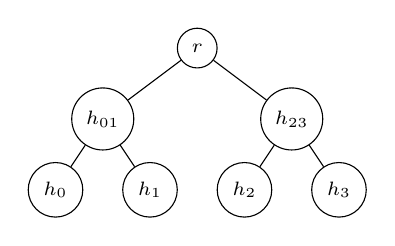
\begin{tikzpicture}[
		level distance=0.9cm,
		level 1/.style={sibling distance=2.4cm},
		level 2/.style={sibling distance=1.2cm},
		every node/.style={font=\scriptsize}
		]
		\node[draw, circle] {$r$}
		child {node[draw, circle] {$h_{01}$}
			child {node[draw, circle] {$h_0$}}
			child {node[draw, circle] {$h_1$}}
		}
		child {node[draw, circle] {$h_{23}$}
			child {node[draw, circle] {$h_2$}}
			child {node[draw, circle] {$h_3$}}
		};
	\end{tikzpicture}
\end{center}
		\begin{pblock}{Uloga}
			Koren stabla je kratka posveta celom nizu; verifikator kasnije traži samo nekoliko vrednosti i autentifikacione putanje.
		\end{pblock}
	\end{frame}
	
	\begin{frame}{Polinom kompozicije}
		\begin{itemize}
			\item AIR može sadržati više ograničenja:
		\end{itemize}
		
		\[
		C_1(X), C_2(X), \ldots, C_k(X)
		\]
		
		\begin{itemize}
			\item Verifikator bira nasumične koeficijente:
		\end{itemize}
		
		\[
		\alpha_1,\alpha_2,\ldots,\alpha_k \in \mathbb{F}
		\]
		
		\begin{itemize}
			\item Dokazivač formira linearnu kombinaciju:
		\end{itemize}
		
		\[
		C(X)=\alpha_1C_1(X)+\alpha_2C_2(X)+\cdots+\alpha_kC_k(X).
		\]
		
		\begin{pblock}{Poenta}
			Umesto mnogo odvojenih provera, verifikator proverava jedan objedinjeni polinomski uslov.
		\end{pblock}
	\end{frame}
	
	\begin{frame}{FRI protokol}
		\begin{pblock}{FRI}
			\textit{Fast Reed-Solomon Interactive Oracle Proof of Proximity} proverava da li je funkcija bliska evaluacijama polinoma niskog stepena.
		\end{pblock}
		
		\begin{itemize}
			\item Nije dovoljno proveriti samo lokalna AIR ograničenja.
			\item Potrebno je proveriti da vrednosti dolaze od jednog konzistentnog polinoma.
			\item FRI rekurzivno smanjuje stepen i domen.
		\end{itemize}
		
		\[
		f_0 \longrightarrow f_1 \longrightarrow f_2 \longrightarrow \cdots \longrightarrow f_r
		\]
		
		\begin{itemize}
			\item Na kraju ostaje mali polinom koji se može direktno proveriti.
		\end{itemize}
	\end{frame}
	
	\begin{frame}{FRI: split-and-fold ideja}
		\begin{itemize}
			\item Polinom se razdvaja na parni i neparni deo:
		\end{itemize}
		
		\[
		f(X)=f_{\mathrm{even}}(X^2)+Xf_{\mathrm{odd}}(X^2)
		\]
		
		\begin{itemize}
			\item Verifikator bira slučajnu vrednost $\beta$.
			\item Dokazivač formira novi polinom:
		\end{itemize}
		
		\[
		g(Y)=f_{\mathrm{even}}(Y)+\beta f_{\mathrm{odd}}(Y).
		\]
		
		\begin{pblock}{Efekat}
			Stepen novog polinoma je približno duplo manji, pa se problem rekurzivno smanjuje.
		\end{pblock}
	\end{frame}
	
	\begin{frame}{DEEP-FRI}
		\begin{itemize}
			\item DEEP znači \textit{Domain Extension for Eliminating Pretenders}.
			\item Ideja: proveravati vrednost i van osnovnog domena.
			\item Verifikator bira tačku $z$ izvan domena i traži:
		\end{itemize}
		
		\[
		f(z)
		\]
		
		\begin{itemize}
			\item Time se dokazivač vezuje za konkretniji polinom.
			\item Zatim se posmatra:
		\end{itemize}
		
		\[
		g(X)=\frac{f(X)-f(z)}{X-z}.
		\]
		
		\begin{pblock}{Poenta}
			DEEP-FRI poboljšava pouzdanost testa, uz zadržavanje efikasnosti FRI pristupa.
		\end{pblock}
	\end{frame}
	
	\begin{frame}{Fiat--Šamir i neinteraktivni dokaz}
		\begin{itemize}
			\item Osnovni protokol se može posmatrati kao interaktivan.
			\item Dokazivač šalje posvete, a verifikator bira slučajne izazove.
			\item Za javno proverljive sisteme potreban je neinteraktivan dokaz.
		\end{itemize}
		
		\begin{pblock}{Fiat--Šamirova heuristika}
			Izazovi se generišu heširanjem prethodnog transkripta.
		\end{pblock}
		
		\[
		\alpha_i = H(x,c_1,c_2,\ldots,c_i)
		\]
		
		\begin{itemize}
			\item Verifikator kasnije ponavlja isto heširanje.
			\item Dokaz može proveriti bilo ko, bez nove interakcije.
		\end{itemize}
	\end{frame}
	
	\begin{frame}{Gde nastaje nulto znanje?}
		\begin{itemize}
			\item AIR, Merkle i FRI proveravaju integritet izračunavanja.
			\item Ali samo po sebi to ne garantuje da se iz upita ne otkriva deo svedoka.
			\item Za zk-STARK potrebno je dodatno maskiranje traga i polinoma.
		\end{itemize}
		
		\begin{pblock}{Razlika}
			\textbf{STARK} proverava da je izračunavanje korektno. \textbf{zk-STARK} dodatno obezbeđuje da dokaz ne otkriva tajne ulaze.
		\end{pblock}
	\end{frame}
	
	% ------------------------------------------------------------
	\section{Primer, poređenje i primene}
	% ------------------------------------------------------------
	
	\begin{frame}{Pojednostavljen primer}
		\begin{itemize}
			\item Početna vrednost je tajna: $x_0$.
			\item Program tri puta računa:
		\end{itemize}
		
		\[
		x_{i+1}=x_i^2+1
		\]
		
		\begin{itemize}
			\item Javni rezultat je $y$.
			\item Treba dokazati da posle tri koraka važi $x_3=y$, bez otkrivanja $x_0$.
		\end{itemize}
		
		\begin{pblock}{AIR ograničenja}
			\[
			x_{i+1}-x_i^2-1=0, \qquad i\in\{0,1,2\}
			\]
			\[
			x_3-y=0
			\]
		\end{pblock}
	\end{frame}
	
	\begin{frame}{zk-SNARK vs. zk-STARK}
		\begin{center}
			\small
			\begin{tabular}{|p{0.27\textwidth}|p{0.29\textwidth}|p{0.29\textwidth}|}
				\hline
				\textbf{Osobina} & \textbf{zk-SNARK} & \textbf{zk-STARK} \\
				\hline
				Podešavanje & često trusted setup & transparentno \\
				\hline
				Dokaz & veoma mali & veći \\
				\hline
				Kriptografska osnova & eliptičke krive, uparivanja & heš funkcije, kodovi \\
				\hline
				Postkvantna sigurnost & uglavnom ne & verovatno da \\
				\hline
				Verifikacija & veoma brza & skalabilna, ali dokaz veći \\
				\hline
			\end{tabular}
		\end{center}
		
		\begin{pblock}{Zaključak}
			zk-SNARK je često bolji kada je veličina dokaza presudna, dok je zk-STARK zanimljiv kada su transparentnost i dugoročna sigurnost važnije.
		\end{pblock}
	\end{frame}
	
	\begin{frame}{Aurora i drugi transparentni sistemi}
		\begin{itemize}
			\item Transparentnost nije osobina isključivo STARK sistema.
			\item Aurora je transparentni zk-SNARK za R1CS instance.
			\item R1CS je sistem ograničenja koji se često koristi za predstavljanje aritmetičkih kola.
		\end{itemize}
		
		\begin{pblock}{Razlika modela}
			Aurora polazi od eksplicitnog aritmetičkog kola, dok STARK prirodnije opisuje dugo izvršavanje programa preko traga izvršavanja i AIR ograničenja.
		\end{pblock}
		
		\begin{itemize}
			\item Zato se sistemi ne porede samo po veličini dokaza.
			\item Važno je i koji model izračunavanja dokazujemo.
		\end{itemize}
	\end{frame}
	
	\begin{frame}{Primene zk-STARK sistema}
		\begin{itemize}
			\item \textbf{Blockchain skaliranje}
			\begin{itemize}
				\item mnogo transakcija se izvršava van osnovnog lanca;
				\item na lanac se šalje dokaz ispravnosti.
			\end{itemize}
			\item \textbf{Proverljivo računanje nad poverljivim podacima}
			\begin{itemize}
				\item medicina, finansije, statistika, regulativa.
			\end{itemize}
			\item \textbf{Identitet i autentifikacija}
			\begin{itemize}
				\item dokaz svojstva bez otkrivanja kompletnog identiteta.
			\end{itemize}
		\end{itemize}
	\end{frame}
	
	\begin{frame}{Prednosti i nedostaci}
		\begin{center}
			\small
			\begin{tabular}{|p{0.43\textwidth}|p{0.43\textwidth}|}
				\hline
				\textbf{Prednosti} & \textbf{Nedostaci} \\
				\hline
				Nema trusted setup faze & Dokazi su obično veći \\
				\hline
				Postkvantna orijentacija & Dokazivač može biti zahtevan \\
				\hline
				Skalabilna verifikacija & Veći memorijski zahtevi \\
				\hline
				Javna proverljivost & Složen izbor parametara \\
				\hline
				Dobar za velika izračunavanja & Nije uvek optimalan za male zadatke \\
				\hline
			\end{tabular}
		\end{center}
	\end{frame}
	
	\begin{frame}{Zaključak}
		\begin{itemize}
			\item zk-STARK omogućava proveru velikih izračunavanja nad poverljivim podacima.
			\item Ključne osobine su transparentnost, skalabilnost i postkvantna orijentacija.
			\item Tehnička osnova su execution trace, AIR, polinomi, Merkle posvete i FRI.
			\item Nulto znanje zahteva dodatno maskiranje, a ne samo proveru integriteta.
			\item U praksi je najvažniji kompromis: veći dokaz, ali manje poverenja u podešavanje i bolja dugoročna sigurnost.
		\end{itemize}
	\end{frame}
	
	\begin{frame}{Ispitna pitanja}
	
	\textbf{Objasniti zašto se zk-STARK sistemi smatraju transparentnim, skalabilnim i verovatno postkvantno sigurnim?}
	
	\textbf{Objasniti osnovni tok zk-STARK sistema i ulogu njegovih ključnih komponenti.}
	
	\end{frame}
	
	\begin{frame}{}
		\small
		\vspace{0.5cm}
		\begin{center}
			\Huge HVALA NA PAŽNJI!
			\\
			\Large Pitanja?
		\end{center}
	\end{frame}
	
\end{document}
